\chapter{Metodología de la Investigación}
\section{Diseño de Investigación}
El presente trabajo adopta un diseño experimental puro, ya que se manipulan variables independientes bajo un control estricto y se miden sus efectos en variables dependientes. Este diseño permite establecer relaciones causales entre las técnicas de procesamiento y análisis de datos y la detección de comportamientos sospechosos.

\subsubsection{Características del Diseño}
\begin{itemize}
    \item \textbf{Tipo de Diseño Experimental:} Diseño de grupos paralelos con \textbf{grupo experimental} y \textbf{grupo control}, seleccionados aleatoriamente a partir del dataset segmentado.
    \item \textbf{Grupos del Diseño:}
    \begin{enumerate}
        \item \textbf{Grupo Experimental:} 
        Aplicación de técnicas avanzadas como YOLOv8, Optical Flow y ConvLSTM para la detección y análisis de comportamientos sospechosos.
        \item \textbf{Grupo Control:} 
        Uso de modelos básicos como SVM o CNN simples, sin técnicas avanzadas de extracción de características ni análisis temporal.
    \end{enumerate}
    \item \textbf{Variables del Estudio:}
    \begin{itemize}
        \item \textbf{Variables Independientes:} Técnicas avanzadas de procesamiento y modelado, como detección de objetos (YOLOv8) y análisis temporal (Optical Flow y ConvLSTM).
        \item \textbf{Variable Dependiente:} Precisión en la detección de comportamientos sospechosos, medida mediante métricas estándar como:
        \begin{itemize}
            \item \textit{Precision (Precisión):} Proporción de predicciones correctas.
            \item \textit{Recall:} Capacidad del modelo para identificar correctamente eventos sospechosos.
            \item \textit{F1-Score:} Balance entre precisión y recall.
            \item \textit{AUC-ROC:} Sensibilidad y especificidad del modelo.
        \end{itemize}
    \end{itemize}
\end{itemize}

\subsubsection{Procedimiento del Diseño}
\begin{enumerate}
    \item \textbf{Asignación de Grupos:} 
    Los videos segmentados y etiquetados se asignarán aleatoriamente a dos grupos:
    \begin{itemize}
        \item \textbf{Grupo Experimental:} Datos procesados con técnicas avanzadas para extracción de características y análisis temporal.
        \item \textbf{Grupo Control:} Datos procesados sin técnicas avanzadas, utilizando modelos básicos para la detección y análisis.
    \end{itemize}
    \item \textbf{Aplicación de Técnicas:}
    \begin{itemize}
        \item Técnicas avanzadas aplicadas en el grupo experimental, incluyendo YOLOv8 para detección de objetos y ConvLSTM para análisis temporal.
        \item Técnicas básicas aplicadas en el grupo control, como SVM y CNN simples.
    \end{itemize}
    \item \textbf{Evaluación:} 
    Se medirá el desempeño de ambos grupos mediante las siguientes métricas:
    \begin{itemize}
        \item Precisión (Accuracy)
        \item Recall
        \item F1-Score
        \item AUC-ROC
    \end{itemize}
    Los resultados serán analizados para determinar diferencias significativas en el desempeño entre los grupos experimental y control.
\end{enumerate}

\subsubsection{Justificación del Diseño}
El diseño experimental puro fue seleccionado debido a su capacidad para:
\begin{itemize}
    \item Establecer relaciones causales entre las técnicas de procesamiento y modelado utilizadas y los resultados en la detección de comportamientos sospechosos.
    \item Controlar variables externas que podrían afectar la validez interna del estudio.
    \item Facilitar la comparación cuantitativa y rigurosa entre el enfoque propuesto y métodos tradicionales, asegurando así un análisis objetivo y replicable.
\end{itemize}





\section{Tipo de Investigación}
El tipo de investigación es correlacional, ya que busca establecer relaciones significativas entre las variables independientes (patrones de comportamiento sospechoso) y la variable dependiente (emisión de alertas). Este tipo es ideal para analizar cómo ciertos comportamientos, como posturas o interacción con objetos, se asocian con eventos delictivos.

\begin{itemize}
    \item Variable Independiente: Patrones detectados (posturas, uso de gorras, movimientos anómalos).
    \item Variable Dependiente: Precisión en la emisión de alertas.
    \item Relación: Se analiza cómo la presencia de ciertos patrones incrementa la probabilidad de comportamientos delictivos.
\end{itemize}

\subsubsection{Ejemplos de aplicaciones correlacionales}
\begin{itemize}
    \item Sultani et al. (2018): Identifican relaciones entre patrones visuales en videos y actividades sospechosas mediante modelos de instancias múltiples.
    \item Zin et al. (2014): Analizan cómo patrones de movimiento correlacionan con eventos delictivos específicos en entornos urbanos.
\end{itemize}

Este enfoque correlacional es esencial para construir modelos predictivos, ya que nos permite identificar variables relevantes para la predicción de delitos, y Reduce el margen de error al basarse en correlaciones estadísticamente significativas.

\section{Enfoque de la Investigación}
El enfoque de esta investigación es cuantitativo, dado que utiliza técnicas numéricas y estadísticas para analizar grandes volúmenes de datos. La visión por computadora, combinada con inteligencia artificial, requiere del procesamiento de datos numéricos para generar resultados objetivos y reproducibles.

\begin{enumerate}
    \item Análisis estadístico y numérico: Se aplican algoritmos de deep learning, como CNN y LSTM, para clasificar y predecir comportamientos.
    \item Métricas de rendimiento: La precisión del sistema se evalúa mediante indicadores como AUC-ROC, precisión, recall y F1-score.
    \item Datos masivos: Los videos de vigilancia generan grandes volúmenes de datos que deben ser procesados de manera eficiente para obtener patrones relevantes.
\end{enumerate}

\subsubsection{Antecedentes del enfoque cuantitativo}
\begin{itemize}
    \item Zaidi et al. (2024): Utilizan CNN para analizar videos, alcanzando precisiones superiores al 90\%, demostrando la capacidad del enfoque cuantitativo para generar resultados precisos.
    \item Buttar et al. (2023): Aplican ConvLSTM para analizar secuencias de video, evidenciando cómo el análisis estadístico mejora la detección de actividades sospechosas.
    \item Patrikar y Parate (2022): Resaltan la importancia del enfoque cuantitativo en el análisis en tiempo real para sistemas de vigilancia basados en edge computing.
\end{itemize}

El aporte del enfoque cuantitativo en esta investigación, proporciona un marco sólido para entrenar modelos predictivos. Tambien garantiza que los resultados sean medibles y comparables y permite validar el sistema en distintos contextos mediante métricas objetivas.

\subsection{Población y Muestra}
\begin{figure}[h] % "h" indica que la imagen se coloque aproximadamente aquí
    \centering
    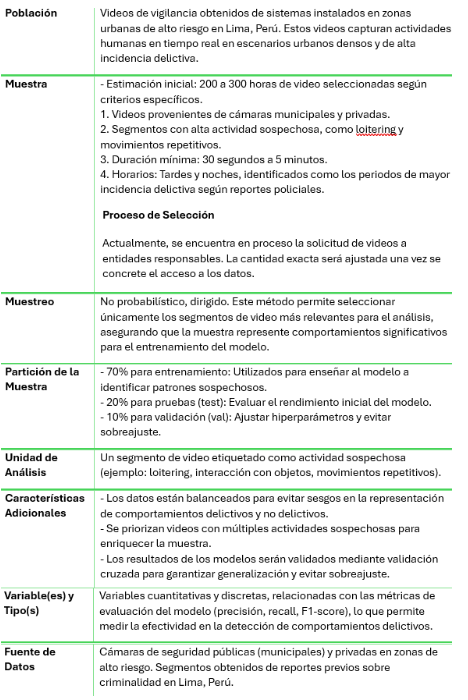
\includegraphics[width=0.7\textwidth]{3/figures/tabla muestra poblacion.png} % Ruta y tamaño de la imagen
    \label{fig:ejemplo} % Etiqueta para referenciar la imagen
\end{figure}